\documentclass{article}

\usepackage[margin=1in]{geometry}
\usepackage{amsmath}
\usepackage{amsfonts}
\usepackage{graphicx}
\usepackage{float}
\usepackage{listings}
\usepackage{color} %red, green, blue, yellow, cyan, magenta, black, white
\definecolor{mygreen}{RGB}{28,172,0} % color values Red, Green, Blue
\definecolor{mylilas}{RGB}{170,55,241}


\title{Homework 3: Digital Control (ECEN 5458)}
\author{Zachary Vogel}
\date{\today}

\newcommand{\rank}{\text{rank}}


\lstset{language=Matlab,%
    %basicstyle=\color{red},
    breaklines=true,%
    morekeywords={matlab2tikz},
    keywordstyle=\color{blue},%
    morekeywords=[2]{1}, keywordstyle=[2]{\color{black}},
    identifierstyle=\color{black},%
    stringstyle=\color{mylilas},
    commentstyle=\color{mygreen},%
    showstringspaces=false,%without this there will be a symbol in the places where there is a space
    numbers=left,%
    numberstyle={\tiny \color{black}},% size of the numbers
    numbersep=9pt, % this defines how far the numbers are from the text
    emph=[1]{for,end,break},emphstyle=[1]\color{red}, %some words to emphasise
    %emph=[2]{word1,word2}, emphstyle=[2]{style},    
}

\begin{document}
\maketitle

\section*{Problem 1}
Problem 5.4 in the book

\subsection*{(a)}
First, do the problem completely in the time domain, by just "chasing" the input signal through the block diagram and plotting the outputs of the zero-order hold (signal u) and the integrator (signal v) as well as the overall output (signal y). Signals u, v, and y are labeled on the block diagram here. Assume zero initial conditions on u and v, so $u(0-)=v(0-)=0$. Let $r(t)$ be such that its samples $r(kT)=0$ at all sampling instants except time $t=0$, when $r(0)=1$.\\


First, let us write out the system equations for the system:
\[r(kT)=\left \{\begin{array}{c}1\quad \text{for}\quad k=0\\0\quad \text{for}\quad k\neq 0\end{array}\right .\]
\[y(kT)=v(kT)+u(kT)\]
\[v(t)=(t-kT)(u(kT)-u(kT-T))\]
\[u(kT)=r(kT)-v(kT)\]

I decided to make a table of the values for the various kTs:
\begin{table}[H]
    \centering
    \begin{tabular}{|l|r|r|r|r|}
        \hline
        time & r & u & v & y\\\hline
        -1   & 0 & 0 & 0 & 0\\\hline
        0   & 1 & 1 & 0 & 1\\\hline
        0.5 & 0 & 1 & 0.5 & 1.5\\\hline
        1   & 0 & 0& 0 & 0\\\hline
        1.5 & 0 & 0 & -0.5 & -0.5\\\hline
        $2^-$   & 0 & 0 & -1 & -1\\\hline
        $2^+$ & 0 & 0 & 0 &0\\\hline
    \end{tabular}
\end{table}

\subsection*{(b)}
Now redo the problem by computing $Y(s)$ then inverting $Y(s)$ to determine $y(t)$.
\subsubsection*{(i)}
For $R^*(s)=R(z)=1$, compute $Y(s)$, the Laplace transform of the output. Work through the diagram in a similar way to what we did in lecture (Lecture 6 19-22). Writing down expressions for $U(s)$ and $V(s)$ may be helpful. The signals $u$ and $v$ are defined in the block diagram in the homework.\\

\[U(s)=(R(s)-V(s))\cfrac{1-e^{-Ts}}{s}\]
\[V(s)=\cfrac{U(s)}{Ts}\]
\[U(s)\left (1+\cfrac{1-e^{-Ts}}{Ts^2}\right )=U(s)\left (\cfrac{Ts^2+1-e^{-Ts}}{Ts^2}\right )\]
\[U(s)=\cfrac{Ts(1-e^{-Ts})}{1+Ts^2-e^{-Ts}}R(s)\]
\[V(s)=\cfrac{1-e^{-Ts}}{1+Ts^2-e^{-Ts}}R(s)\]
\[Y(s)=(1+Ts)\cfrac{1-e^{-Ts}}{Ts^2+1-e^{-Ts}}R(s)\]

\subsubsection*{(ii)}
Invert $Y(s)$. Carefully explain how you do this. Do you get the same response as in part $(a)$ above?\\

I couldn't figure out how to invert this. If I used a different substitution like for instance the inverse of the backwards substitution rule, maybe I would get a better transfer function.


\section*{Problem 2}
Given the mapping $z=e^{sT}$ show two things.
\subsection*{(a)}
Show that vertical lines in the s plane map to circles in the z-plane.\\

Vertical lines in the s plane are defined by $s=c_1+j\omega$, where $c_1$ is constant. This translates to $z=e^{c_1T}e^{j\omega T}=k_1e^{j\omega T}$. Thus all vertical lines map to a constant times the unit circle. This is important because any poles left of the line $s=j\omega$ in the s plane are stable and, since this line maps to the unit circle in the z plane, any poles inside the unit circle will also be stable (assuming T=1).
\subsection*{(b)}
Show that horizontal lines in the s plane mape to radial lines in the z-plane.\\

Horizontal lines in the s plane are defined $s=\alpha+jc_2$, where $c_2$ is constant. This translates to $z=e^{\alpha T}e^{jc_2 T}$. This creates a line that points out from the origin at angle $c_2 T$ in both directions.

\section*{Problem 3}
Problem 6.3 from the book where $\omega_1=3\frac{rad}{s}$.\\
For:
\[H(s)=\cfrac{s+1}{0.1s+1}\]
For each of the following desgin methods compute and plot in the z-plane the pole and zero locations and compute the amount of phase lead given by the equivalent network $z_1=e^{j\omega_1T}$ if $T=0.25$ sec and the design is via.\\

Note I did most of this problem in Matlab. The code is in the appendix.
\subsection*{(i)}
Forward Rectangular Rule\\
This gives:
\[H(z)=\cfrac{z-0.75}{0.1z+0.15}\]
The frequency response was: $0.7783+2.8167j$. The pz map of the system is:
\begin{figure}[H]
    \centering
    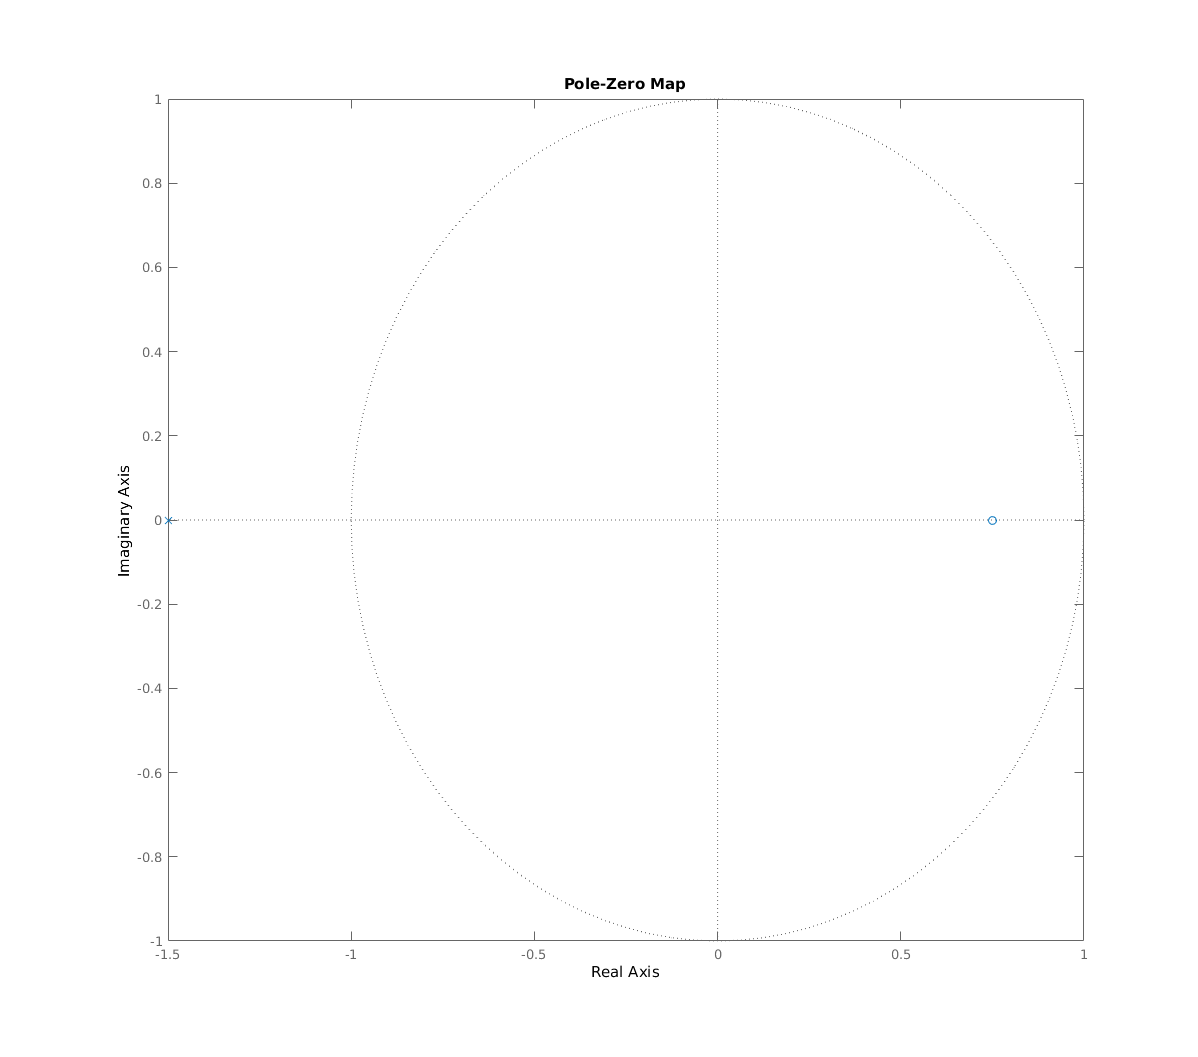
\includegraphics[width=0.6\textwidth]{PR3_1.png}
\end{figure}

\subsection*{(ii)}
Backward Rectangular Rule\\
This gives:
\[H(z)=\cfrac{1.25z-1}{0.35z-0.1}\]
TThe frequency response was: $2.3359+1.8869j$. The pz map of the system is:
\begin{figure}[H]
    \centering
    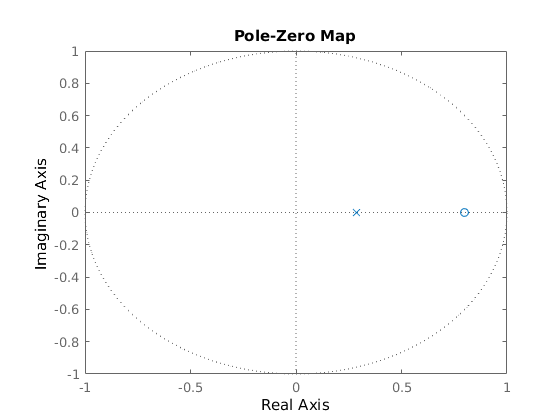
\includegraphics[width=0.6\textwidth]{PR3_2.png}
\end{figure}

\subsection*{(iii)}
Bilinear rule\\
This gives:
\[H(z)=\cfrac{9z-7}{1.8z+0.2}\]
The frequency response was: $1.8119+2.5784j$. The pz map of the system is:
\begin{figure}[H]
    \centering
    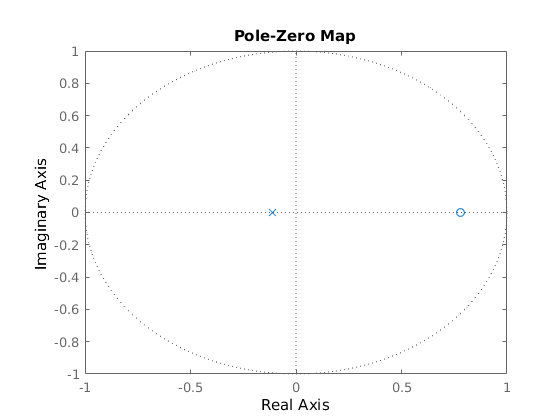
\includegraphics[width=0.6\textwidth]{PR3_3.png}
\end{figure}
\subsection*{(iv)}
Bilinear rule with prewarping at $\omega_1$\\
This gives:
\[H(z)=\cfrac{8.6214z-6.6214}{1.76214z+0.23786}\]
The frequency response was: $1.7431+2.4771j$. The pz map of the system is:
\begin{figure}[H]
    \centering
    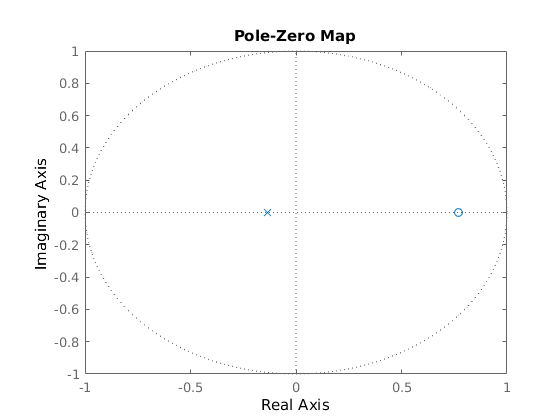
\includegraphics[width=0.6\textwidth]{PR3_4.png}
\end{figure}
\subsection*{(v)}
Zero-pole mapping\\
This gives:
\[H(z)=\cfrac{z-e^{-0.25}}{10(z-e^{-2.5})}\]
The frequency response was: $0.0490+0.0536j$. The pz map of the system is:
\begin{figure}[H]
    \centering
    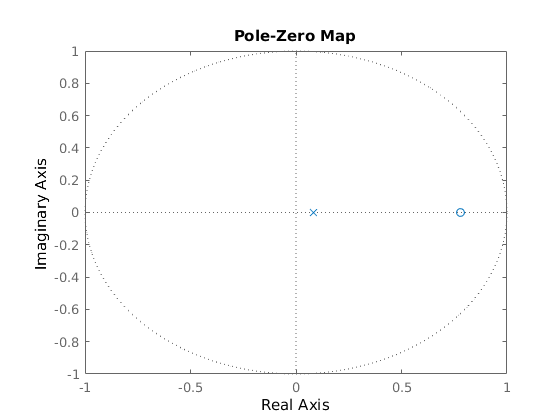
\includegraphics[width=0.6\textwidth]{PR3_5.png}
\end{figure}

\subsection*{(vi)}
Zero-order-hold equivalent\\
\[H(z)=\cfrac{z-1}{z}\mathcal{Z}\left (\cfrac{s+1}{0.1s^2+s}\right )=\cfrac{z-1}{z}\mathcal{Z}\left (\cfrac{1}{s}+\cfrac{9}{s+10}\right)\]
\[H(z)=\cfrac{2z-1+e^{-2.5}}{z-e^{-2.5}}\]
The frequency response was: $1.4477+0.5795j$. The pz map of the system is:
\begin{figure}[H]
    \centering
    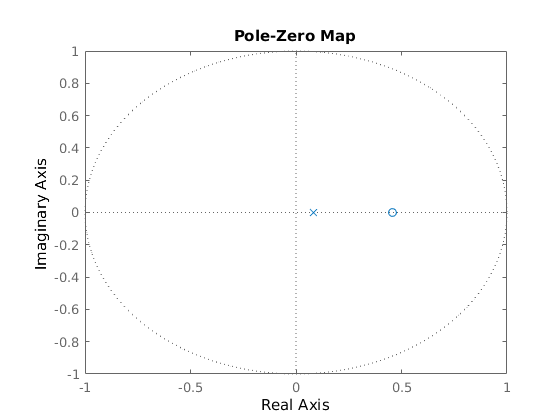
\includegraphics[width=0.6\textwidth]{PR3_6.png}
\end{figure}

\subsection*{(vii)}
Triangular-hold equivalent\\
\[H(z)=\cfrac{(z-1)^2}{Tz}\mathcal{Z}\left(\cfrac{s+1}{s^2(0.1s+1)}\right)=\cfrac{(9z-1)(z-e^{-2.5})+0.25(z-e^{-2.5})-9(z-1)^2}{Tz(z-e^{-2.5})}\]
The frequency response was: $46.6057+23.1541j$. The pz map of the system is:
\begin{figure}[H]
    \centering
    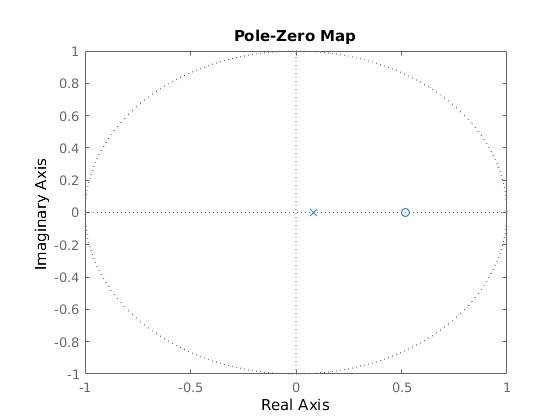
\includegraphics[width=0.6\textwidth]{PR3_7.png}
\end{figure}

\subsection*{(Part b)}
Plot over the frequency range $\omega_l=0.1\to\omega_h=100$ the amplitude and phase Bode plots for each of the above equations.\\
Here are all the bode plots for each of the above:
Part 1:
\begin{figure}[H]
    \centering
    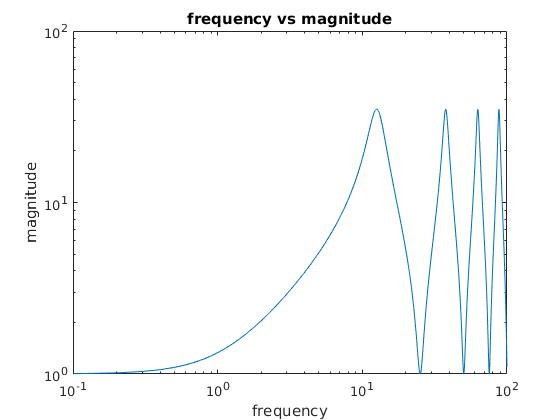
\includegraphics[width=0.8\textwidth]{PR3_amp.png}
\end{figure}
\begin{figure}[H]
    \centering
    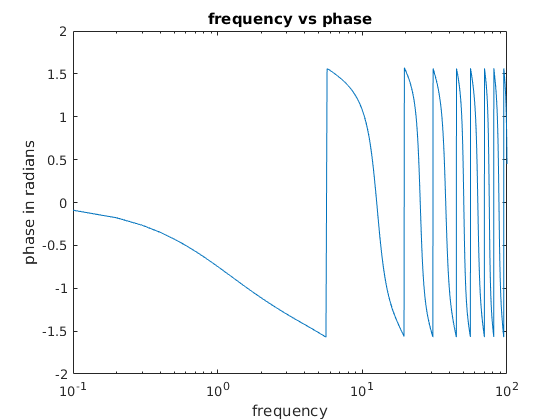
\includegraphics[width=0.8\textwidth]{PR3_1phase.png}
\end{figure}
Part 2:
\begin{figure}[H]
    \centering
    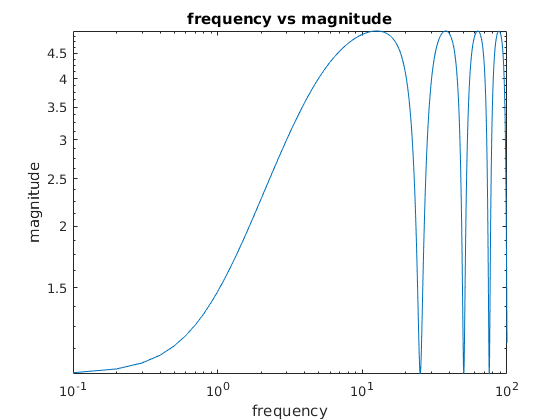
\includegraphics[width=0.8\textwidth]{PR3_2amp.png}
\end{figure}
\begin{figure}[H]
    \centering
    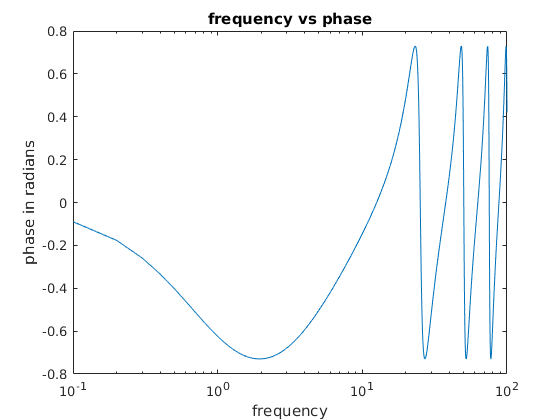
\includegraphics[width=0.8\textwidth]{PR3_2phase.png}
\end{figure}
Part 3:
\begin{figure}[H]
    \centering
    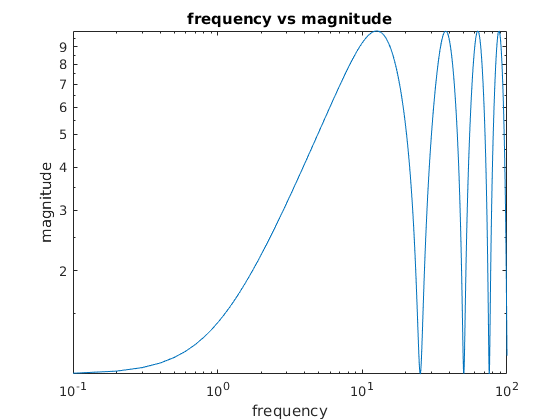
\includegraphics[width=0.8\textwidth]{PR3_3amp.png}
\end{figure}
\begin{figure}[H]
    \centering
    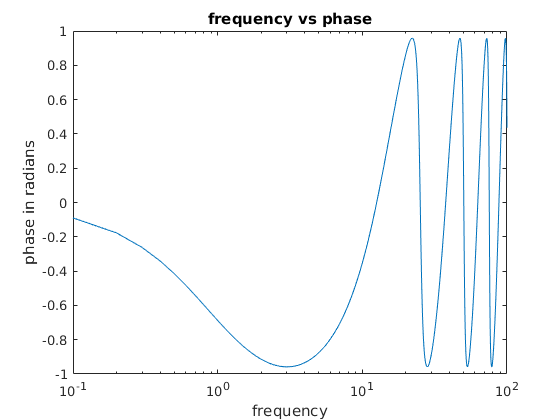
\includegraphics[width=0.8\textwidth]{PR3_3phase.png}
\end{figure}
Part 4:
\begin{figure}[H]
    \centering
    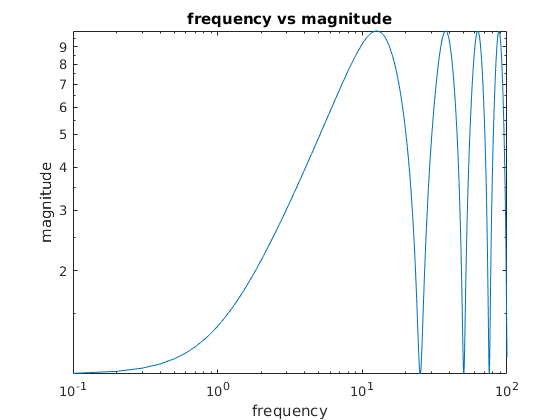
\includegraphics[width=0.8\textwidth]{PR3_4amp.png}
\end{figure}
\begin{figure}[H]
    \centering
    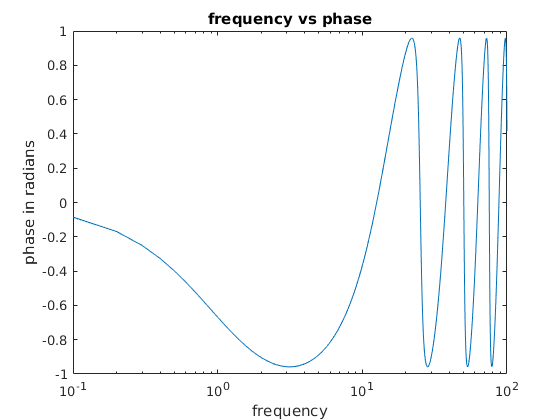
\includegraphics[width=0.8\textwidth]{PR3_4phase.png}
\end{figure}
Part 5:
\begin{figure}[H]
    \centering
    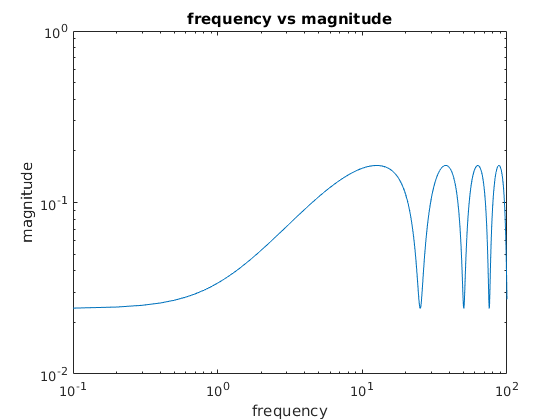
\includegraphics[width=0.8\textwidth]{PR3_5amp.png}
\end{figure}
\begin{figure}[H]
    \centering
    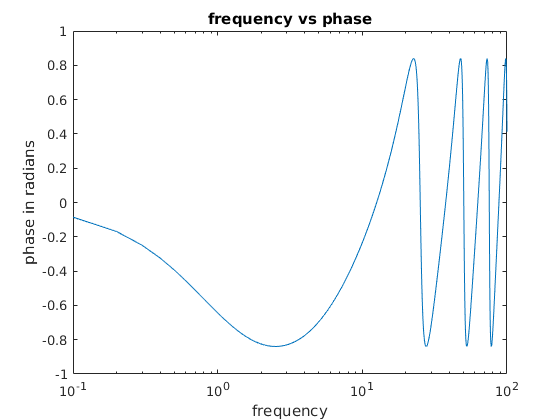
\includegraphics[width=0.8\textwidth]{PR3_5phase.png}
\end{figure}
Part 6:
\begin{figure}[H]
    \centering
    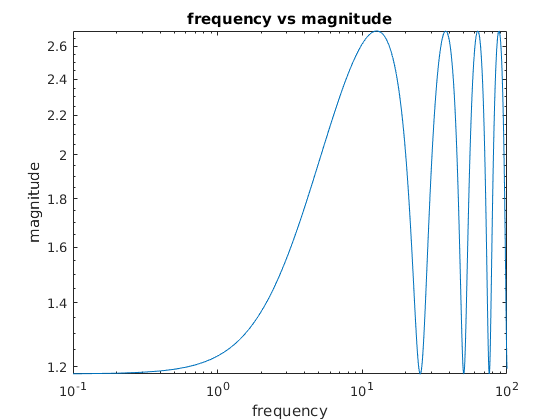
\includegraphics[width=0.8\textwidth]{PR3_6amp.png}
\end{figure}
\begin{figure}[H]
    \centering
    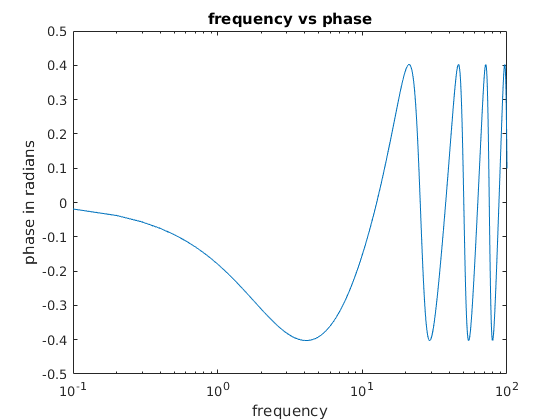
\includegraphics[width=0.8\textwidth]{PR3_6phase.png}
\end{figure}
Part 7:
\begin{figure}[H]
    \centering
    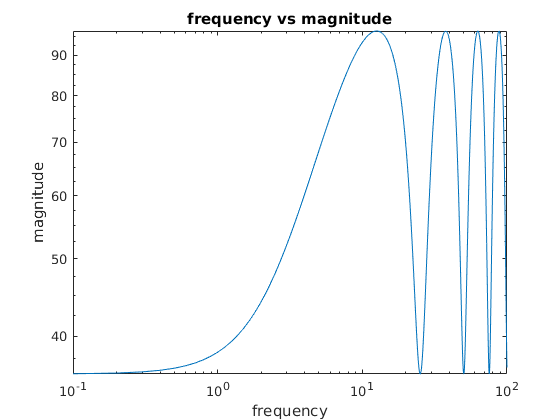
\includegraphics[width=0.8\textwidth]{PR3_7amp.png}
\end{figure}
\begin{figure}[H]
    \centering
    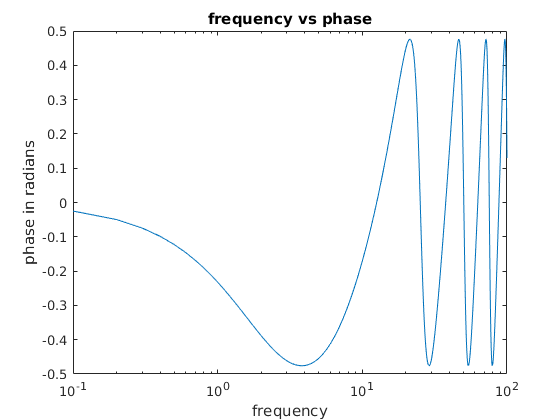
\includegraphics[width=0.8\textwidth]{PR3_7phase.png}
\end{figure}

I couldn't figure out if I did something wrong or the phase and bode plots actually looked like that.

\section*{Problem 4}
Consider the continuous time transfer function:
\[H(s)=\cfrac{1}{(s+a)(s+b)}\]
Assume a sample period of T seconds for all parts of the problem.
\subsection*{(a)}
Find the discrete-equivalent $H(z)$ using pole-zero mapping, where one zero at infinity is mapped to infinity, and where the DC-gain of $H(z)$ is matched with that of $H(s)$.\\

Since there is only one zero for the system at infinity, our discrete transfer function is:
\[H(z)=K\cfrac{1}{(z-e^{-aT})(z-e^{-bT})}\]
where $K=\frac{(1-e^{-aT})(1-e^{-bT})}{b*a}$.


\subsection*{(b)}
Find the discrete-equivalent $H(z)$ using the trapezoid-rule (without prewarping).\\

Here we substitute $s=\cfrac{2(z-1)}{T(z+1)}$ to get:
\[H(z)=\cfrac{T(z+1)}{(2(z-1)+aT(z+1))(2(z-1)+bT(z+1))}=\cfrac{T}{(2+aT)(2+bT)}\cfrac{(z+1)}{(z+\frac{aT-1}{2+aT})(z+\frac{bT-1}{2+bT})}\]

\subsection*{(c)}
Find the discrete-equivalent $H(z)$ using the zero-order-hold (ZOH) equivalent.\\

Start with the equation for zero-order holds:
\[H(z)=\cfrac{z-1}{z}\mathcal{Z}\left (\cfrac{1}{s(s+a)(s+b)}\right )\]
Now use partial fraction expansion on $H(s)$:
\[H(s)=\cfrac{A}{s}+\cfrac{B}{s+a}+\cfrac{C}{s+b}\implies\quad A(s^2+(b+a)s+b*a)+B(s^2+bs)+C(s^2+as)=1\]
This implies that $A=\frac{1}{b*a}$, $B=\frac{1}{a^2-ba}$, and $C=\frac{1}{b^2-ab}$. This gives:
\[H(z)=\cfrac{1}{ab}+\cfrac{z-1}{(a^2-ab)(z-e^{-aT})}+\cfrac{z-1}{(b^2-ab)(z-e^{-bT})}\]

\subsection*{(d)}
For each part, a, b, and c above, determine whether there are any bounds (and if so, provide them) on the plant parameters a and b as well as the sample period T for a bounded-input bounded-output stability of $H(z)$. In other words, for each discrete-equivalent function, find a, b and T that make the transfer function, $H(z)$ BIBO unstable.\\

Assuming all the constants are positive, the pole-zero mapping can't ever be BIBO unstable. The poles will be at worst marginally stable with magnitude 1 unless a and b are negative in which case the system is at best marginally stable.\\

The trapezoid rule function follows the same pattern, with the system always being stable for positive a and b. The system begins to be marginally stable when $aT<=-0.5$ or $bT<=-0.5$.\\

The ZOH transfer function follows the same rules as the pole-zero mapping transfer function. Positive a and b give stability, negative a or b give marginal stability or instability.


\section*{Problem 5}
Converting a continuous transfer function to a discrete one using a zero-order hold involves using the equations:
\[G(z)=\cfrac{z-1}{z}\mathcal{Z}\left \{\cfrac{G(s)}{s}\right \}\]
A similar equation can be found for a first-order hold, answer the following questions.
\subsection*{(a)}
Derive the simple formula which yields the effect of a first-order hold digital-to-analog converter on the continuous transfer function. Simplify as much as possible.\\

First, let's right out the transfer function for a first-order hold:
\[H(s)=\cfrac{1+Ts}{Ts^2}(1-e^{-sT})^2\]
Now let us do some stuff:
\[G(z)=\mathcal{Z}\left ( \cfrac{1+Ts}{Ts}(1-e^{-Ts})\right )(1-z^{-1})\mathcal{Z}\left (\cfrac{G(s)}{s}\right )\]
\[G(z)=(1-z^{-1})^2\mathcal{Z}\left (\cfrac{1+Ts}{Ts^2}G(s)\right )\]


\subsection*{(b)}
When using a FOH as in Figure 2, if the plant $G(s)=\frac{s}{s+1}$, then what is $G(z)$? Use the formula from part a to solve for $G(z)$. Express $G(z)$ as simply as possible.\\

Finding $G(z)$ we get:
\[G(z)=(1-z^{-1})^2\mathcal{Z}\left (\cfrac{\frac{1}{T}+s}{s(s+1)}\right )=(1-z^{-1})^2\mathcal{Z}\left (\cfrac{1}{Ts}+\cfrac{T-1}{T(s+1)}\right )\]
\[G(z)=(1-z^{-1})^2\left (\cfrac{z}{T(z-1)}+\cfrac{z}{z-e^{-T}}-\cfrac{z}{T(z-e^{-T})}\right )=\cfrac{z-1}{Tz}+\left (1-\cfrac{1}{T}\right )\cfrac{(z-1)^2}{z(z-e^{-T})}\]

\subsection*{(c)}
Suppose that in addition to the assumptions from above the sampling period is $T=1$, then what is $G(z)$? That is, what is the transfer function $G(z)$ from $u(kT)$ to $y(kT)$ in figure 2 when $G(s)=\frac{s}{s+1}$ and the sample period is $T=1$ second?\\

Given $T=1$ the problem simplifies greatly to:
\[G(z)=\cfrac{z-1}{z}\]

\subsection*{(d)}
Assuming the assumptions from the previous parts, what is the unit step response of $G(z)$? That is for $G(s)=\frac{s}{s+1}$, a sample period of $T=1$, and a unit step input $u(kT)=1(kT)$, then what is $y(kT)$?\\

Given those conditions, the trasnfer function $Y(z)$ will be:
\[Y(z)=\cfrac{z-1}{z}\cfrac{z}{z-1}=1\]
which yields the unit impulse response for $y(kT)$.
\[y(kT)=\left \{\begin{array}{l}1\quad \text{for}\quad k=0\\0\quad  \text{else}\end{array}\right .\]

\section*{Problem 6}
In class it was noted that one can fully analyze sampled data systems using continuous time techniques, specifically the Laplace Transform, when properly modeling the impulse response of various discrete effects. For instance, a zero order hold can be described as:
\[ZOH(s)=\cfrac{1-e^{-sT}}{s}\]
and the error as:
\[e*(t)=\sum_{k=-\infty}^{\infty}e(t)\delta (t-kT)\]
where $\delta(t)$ is the continuous-time impulse function, k is the sample index, and T is the sample period.
\subsection*{(a)}
If $G(s)=\frac{a}{s}$ for some constant $a$, what is the discrete-time $G(z)$ representation of teh plant $G(s)$ preceded by a ZOH and followed by a sampler.\\

Simply using the equation $G(z)=\cfrac{z-1}{z}\mathcal{Z}(\frac{G(s)}{s})$ we get:
\[G(z)=\cfrac{z-1}{z}\cfrac{aTz}{(z-1)^2}=\cfrac{aT}{z-1}\]

\subsection*{(b)}
Suppose the following PD controller is used:
\[D(z)=K+KT_D\cfrac{z-1}{z}\]
where the gains $K$ and $T_D$ can be adjusted independently. If the above controller is $D(z)$ find $D^*(s)$.\\

Given that $D^*(s)=D(z)\bigg|_{z_0=e^{s_0T}}$ we get:
\[D^*(s)=K+KT_D\cfrac{s}{s+\infty}\]
Realistically, the infinity is set to a number that is orders of magnitude bigger than any poles in the system.

\subsection*{(c)}
Given the closed loop diagram in figure 3 of the homework set, assume $G(s)=\frac{a}{s}$ as in part (a) and assume the compensator $D^*(s)$ as determined in part (b).\\
Let
\[y(kT)=y(t)\bigg|_{t=kT}\]
be samples of $y(t)$, and let
\[r(kT)=r(t)\bigg|_{t=kT}\]
be samples of $r(t)$.\\
With $Y(z)$ being the z-transform of $y(kT)$ and $R(z)$ being the z transform of $r(kT)$, compute the transfer function $\frac{Y(z)}{R(z)}$.\\

Here we just use our existing $G(z)$ and $D(z)$ to find the transfer function:
\[\cfrac{Y(z)}{R(z)}=\cfrac{1}{1+G(z)D(z)}=\cfrac{1}{1+\cfrac{aTz+Kz(z-1)+KT_D(z-1)^2}{z(z-1)}}=\cfrac{z(z-1)}{z^2-z+aTz+Kz^2-Kz+KT_D(z-1)^2}\]
This simplifies to:
\[\cfrac{Y(z)}{R(z)}=\cfrac{z(z-1)}{(K+1+KT_D)z^2-z(2KT_D+K+1-aT)+KT_D}\]

\subsection*{(d)}
Again, assume $G(s)$ and $D*(s)$ as above for the closed-loop block diagram on the previous page. Now, let the various plant and control parameters be $T=\frac{3}{4}$, $a=1$, $K=1$, and $T_D=\frac{1}{4}$.\\
If $r(t)$ is such that its samples are:
\[r(kT)=\left \{\begin{array}{c}1,\quad k=0\\0, \quad k\neq 0\end{array}\right .\]
determine the samples $y(kT)$ of the output $y(t)$.\\

Noting that $R(z)=1$, we get:
\[Y(z)=\cfrac{z(z-1)}{2.25z^2-1.75z+0.25}\]
Let's do some partial fraction expansion:
\[Y(z)=\cfrac{1}{2.25}\cfrac{z^2-z}{z^2-\frac{1.75}{2.25}z+\frac{0.25}{2.25}}=\cfrac{1}{2.25}\cfrac{z^2-z}{(z+0.5892)(z+0.1886)}=\cfrac{1}{2.25}=\cfrac{4}{9}\left( 1+\cfrac{-\frac{2}{9}z-\frac{1}{9}}{(z+0.5892)(z+0.1886)}\right )\]
\[Y(z)=\cfrac{4}{9}\left (1+\cfrac{A}{z+0.5892}+\cfrac{B}{z+0.1886}\right )\]
\[A+B=-\frac{2}{9}\quad 0.1886A+0.5892B=-\frac{1}{9}\]
This leads to $A=-0.0495$ and $B=-0.1727$. Thus we can find $y(kT)$:
\[y(kT)=\cfrac{4}{9}\left (\delta(kT)-0.0495(-0.5892)^{k-1}1(kT-T)-0.1727(-0.1886)^{k-1}1(kT-T)\right )\]
This isn't in the proper form to display it, but this is an exponentially decaying sinusoid. I know this because negative constants with magnitude raised to one will eventually converge to 0 when raised to ever increasing powers.

\subsection*{(e)}
Assuming everything is the same again, determine $Y(s)$ for the closed-loop block diagram on the previous page. Be as explicit as possible (don't need $y(t)$).\\
I ran out of time right here. Wasn't sure if I should use $s=\frac{\ln(z)}{T}$ or something else to convert.


\section*{Problem 7}
Consider a second-order discrete-time system and sampling times of $T=0.1$, $T=0.25$, and $T=0.75$ seconds.
\subsection*{(a)}
For each sampling rate, plot the acceptable region for the poles of the second-order system in the z-plane such that the following dynamic step response specifications would be satisfied:
\begin{itemize}
    \item $t_r<0.5$ seconds
    \item overshoot less than $25\%$
    \item $t_s<2.5$ seconds
\end{itemize}
Assume the rise time $t_r$ is defined as the time elapsed from when the response is $10\%$ to $90\%$ of its steady-state value, and the settling time $t_s$ is defined as the time after which the response remains within $1\%$ of its steady-state value.\\

A standard second order system is of the form:
\[H(s)=\cfrac{\omega_n^2}{s^2+2\zeta\omega_ns+\omega_n^2}\]
\[\sigma=\zeta\omega_n\]
\[\omega_d=\omega_n\sqrt{1-\zeta^2}\]
with poles at $s_p=-\sigma\pm j\omega_d$. The conditions on the continuous transfer function give:
\[t_r\geq \cfrac{1.8}{\omega_n}\]
\[M_p\geq 1-\cfrac{\zeta}{0.6}\]
\[t_s\geq \cfrac{4.6}{\zeta\omega_n}\]
Thus, $\omega_n\geq \frac{1.8}{t_r}=3.6$, $\zeta\geq 0.6(1-M_p)=0.45$, and $\zeta\omega_n\geq\frac{4.6}{t_s}=1.84$. Since we know that the discrete poles are:
\[z=e^{sT}=e^{-\zeta\omega_nT}e^{\pm j\omega_n\sqrt{1-\zeta^2}T}\]
we can now plot the regions for various sampling times in Matlab. The code for this problem is in the appendix. The graphs are for the various sampling rates are shown below.
\begin{figure}[H]
    \centering
    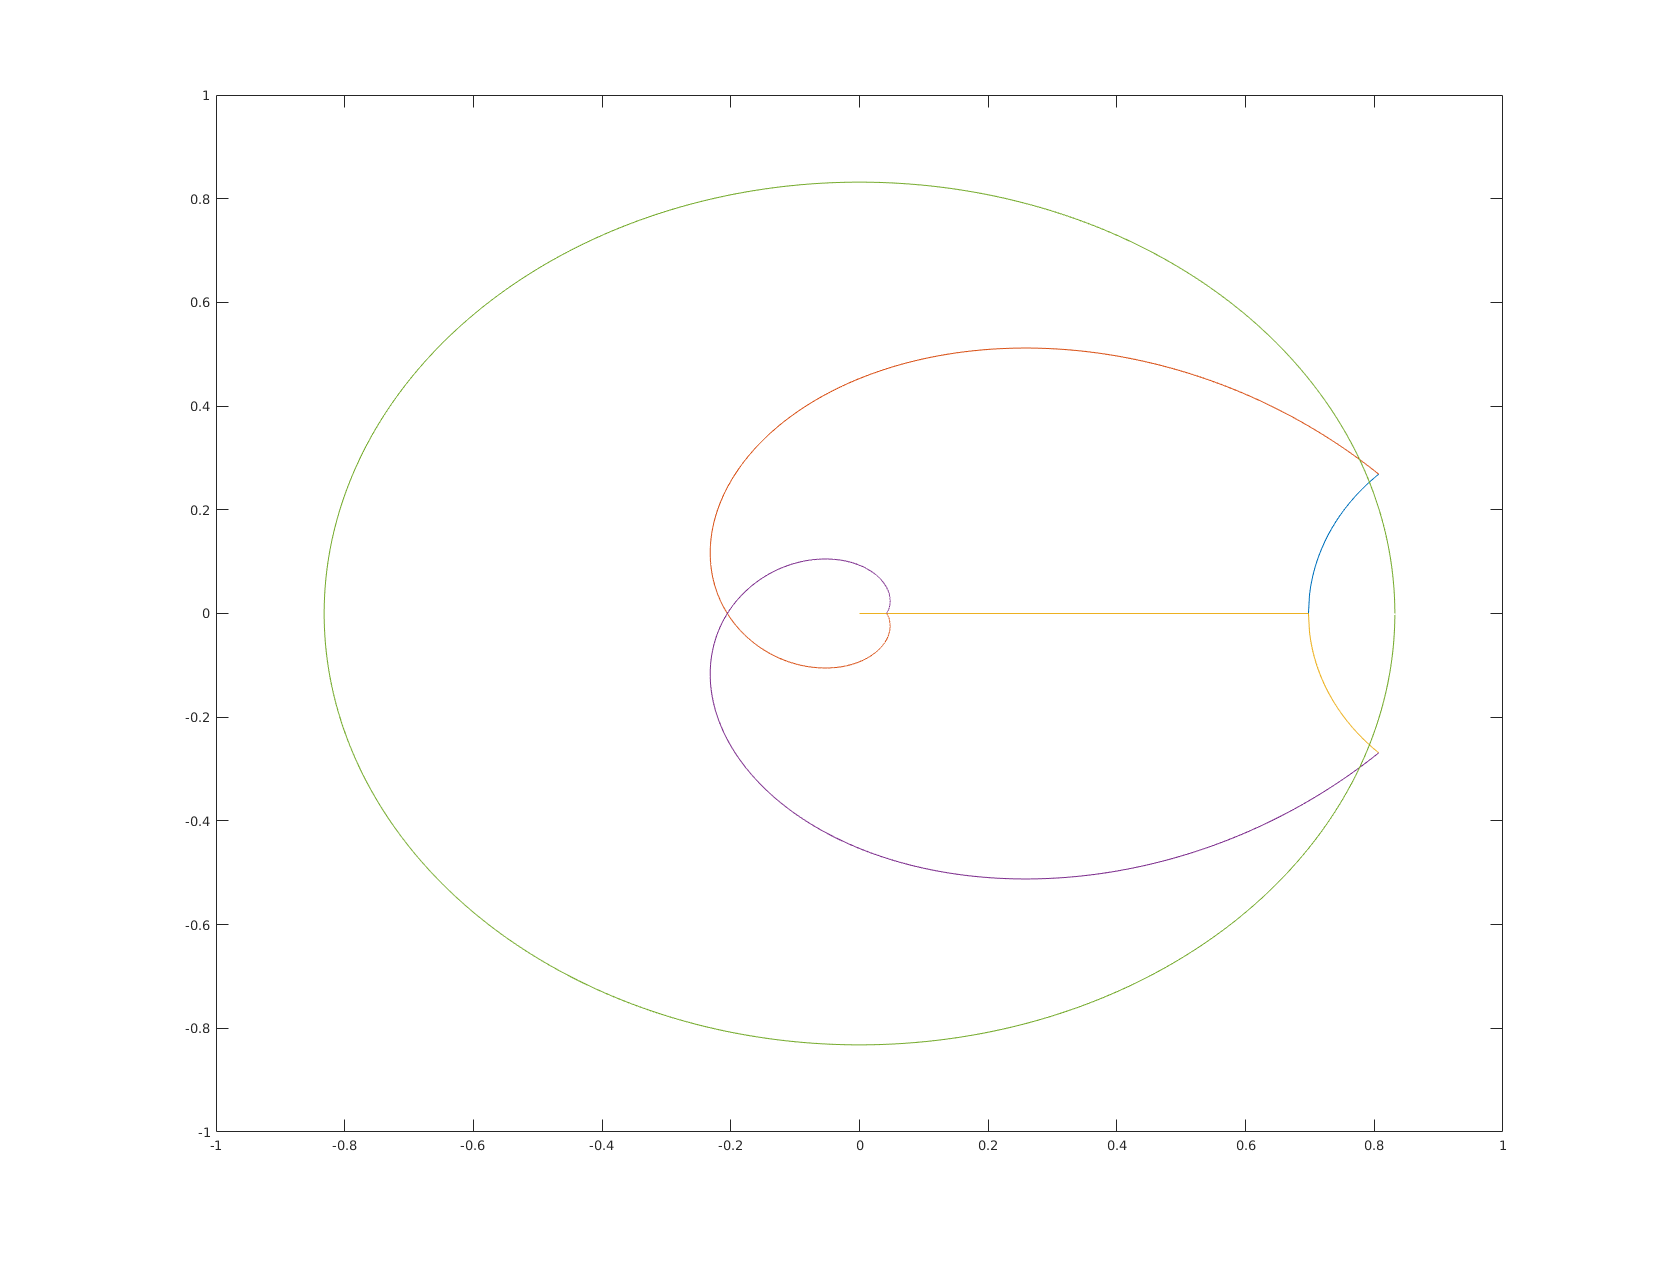
\includegraphics[width=0.8\textwidth]{Pr7_t1.png}
    \caption{The acceptable region for our constraints with a sampling period of $T=0.1$}
\end{figure}
\begin{figure}[H]
    \centering
    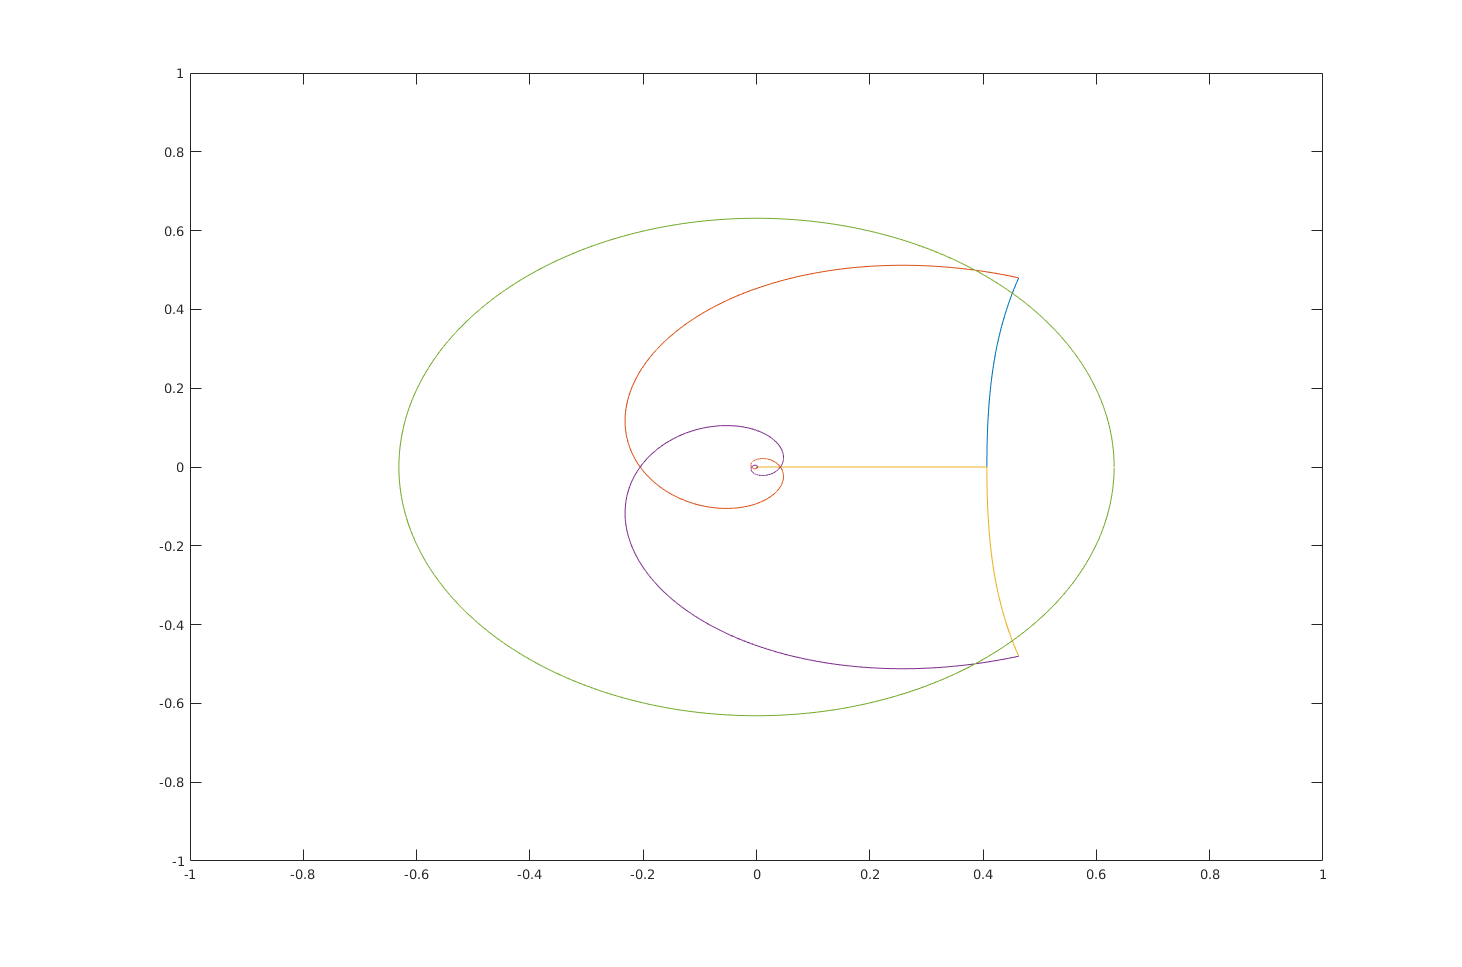
\includegraphics[width=0.8\textwidth]{PR7_t25.png}
    \caption{The acceptable region for our constraints with a sampling period of $T=0.25$}
\end{figure}
\begin{figure}[H]
    \centering
    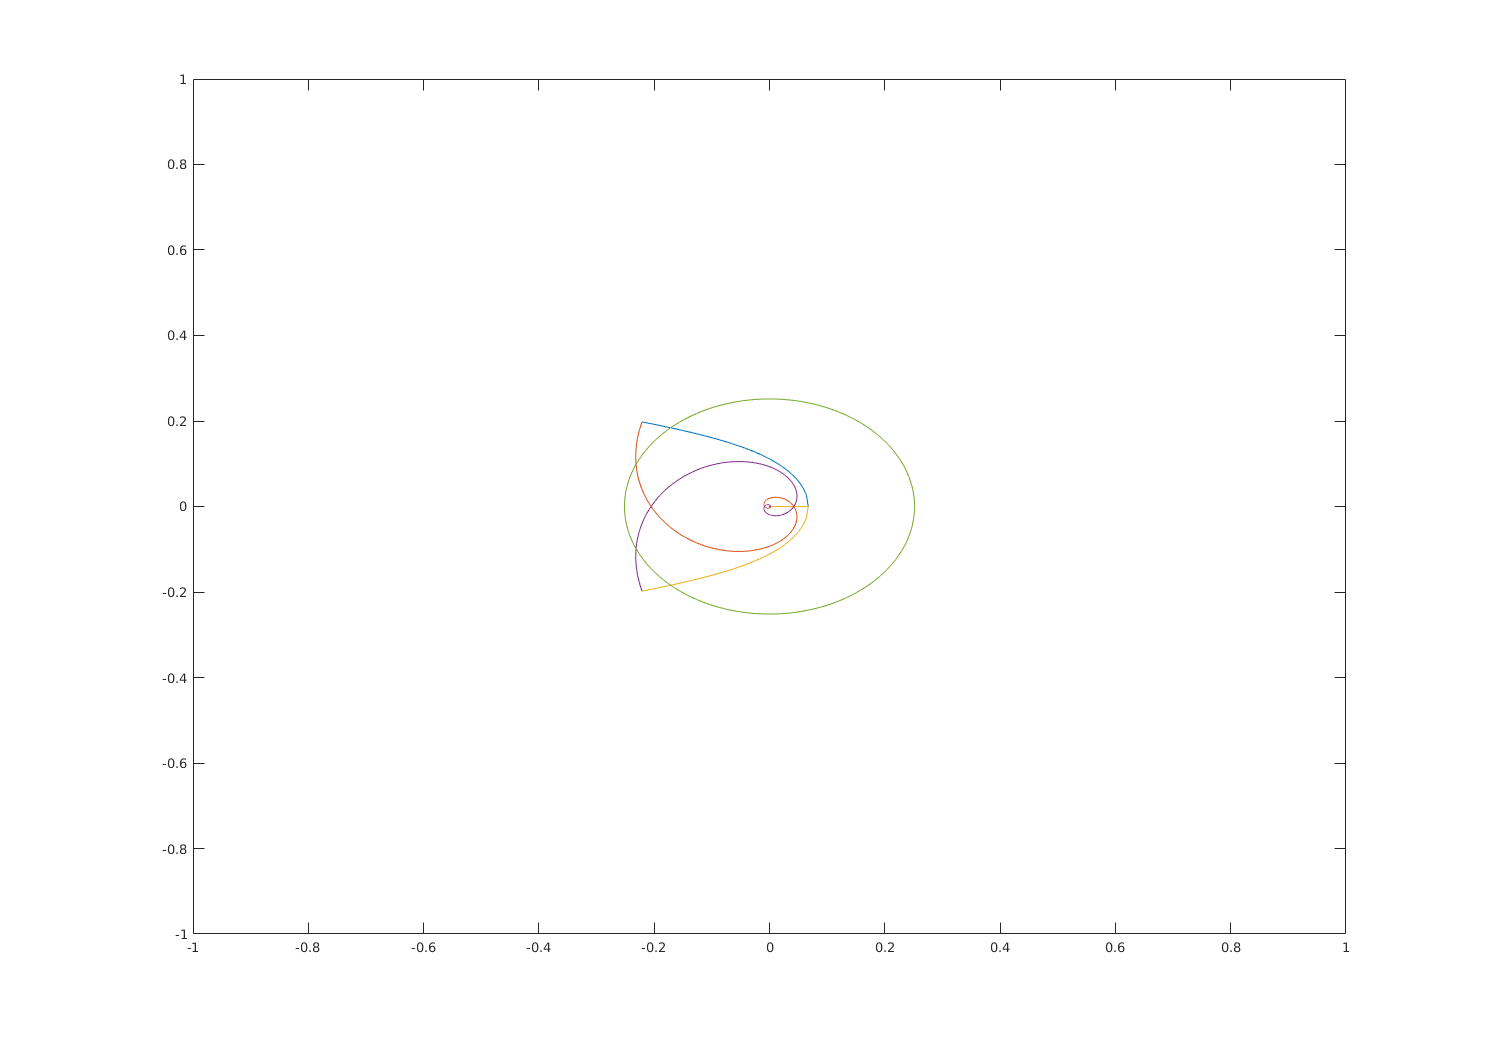
\includegraphics[width=0.8\textwidth]{PR7_t75.png}
    \caption{The acceptable region for our constraints with a sampling period of $T=0.75$. Note that this plot seemed to flip over the origin.}
\end{figure}
I apoligize for not filling in the area, but I am not actually aware of how to do that.

\subsection*{(b)}
How does the sampling rate affect the size of the "acceptable region" and hence the ability to solver for an appropriate compensator to meet specifications?\\

As is clearly seen in the graphs, the higher the sampling rate the smaller the area of convergence. Considering system performance generally degrades with higher sampling rate this makes pretty clear sense. Thus, raising the sample rates means one has to build a better controller/compensator for the system, but that cost is made up in less CPU utilization.

\subsection*{(c)}
How would an additional zero affect the step response? How should the "acceptable region" that was plotted in the z-plane be altered if there is an additional zero?\\

Adding an additional stable non-zero is like adding a derivative term on the system. If the initial step response is $x(t)$, the response with an added zero will be $x(t)+k\dot{x}(t)$ where $k$ is determined by the location of the pole. This extra term will increase the overshoot of the system, while decreasing the rise time. This means the acceptable region could get larger or smaller depending on what was the main constraint of the original system. If the rise time was a problem, adding
a derivative term will help by making it rise faster, but if overshoot was the problem it will almost certainly get worse.


\subsection*{(d)}
How would an additional pole affect the step response? How should the "acceptable region" that was plotted in the z-plane be altered if there is an additional pole?\\

Adding a stable pole to the system will have add another exponentially deccaying term to the system. In this case, the rise time of the system must go up because we have another exponential term that must decay before reaching the steady-state value. This also means that the affect on the acceptable region will be a reduction in size of that region. Specifically, the area corresponding to rise time will go down.

\appendix
\section*{Code Appendix}
Problem 3
\lstinputlisting{pr3.m}
Problem 7
\lstinputlisting{pr7.m}

\end{document}
